\section{Testing}
During the development of the application we have had great success working test oriented.
In particular when developing the conversion from abstract syntax tree to control flow graph, testing has been invaluable.
The abstract nature of the syntax tree together with the many possibilities of python yield a huge number of cases for each construct, and the edges have to be just right in every one of them.

When developing all these fragments of the complete grammar, we need to be sure that our previous work still works as intended.
To help us be sure that all our assumptions and implementations hold we have utilised unit testing a great deal.
The following will mention some of the issues where testing has helped the process.

\paragraph{Cases}
An example of a construct which has many different cases is the \texttt{if} control structure, which has variants with \texttt{elif} and \texttt{else} statements.
The \texttt{if} abstract syntax node contains an \emph{orelse} reference which can either be another \texttt{if}, representing an \text{elif} clause, or a list of statements, representing the body of an \texttt{else} clause.
In addition an \texttt{if} can have many different expressions in its \emph{test} clause.
These expressions are often logic expressions but can also be nameconstants, function calls, lambdas and even a list.
To illustrate the three d\texttt{if}ferent cases three abstract directed graphs have been made.
\begin{itemize}
\item The graph for a single \texttt{if} statement can be seen on the left on \cref{test:ast:if_and_else}.
\item The graph for an \texttt{if} and an \texttt{elif} statement can be seen on the right on \cref{test:ast:if_and_else}.
\item The graph for an \texttt{if}, \texttt{elif} and else statement can be seen on \cref{test:ast:if_elif_else}
\end{itemize}
\textbf{Note:} On \cref{test:ast:if_and_else} and \cref{test:ast:if_elif_else}, \textit{expr} is an expression and \textit{stmt*} is a list of statements.


\begin{figure}
    \begin{subfigure}[b]{0.45\textwidth}
        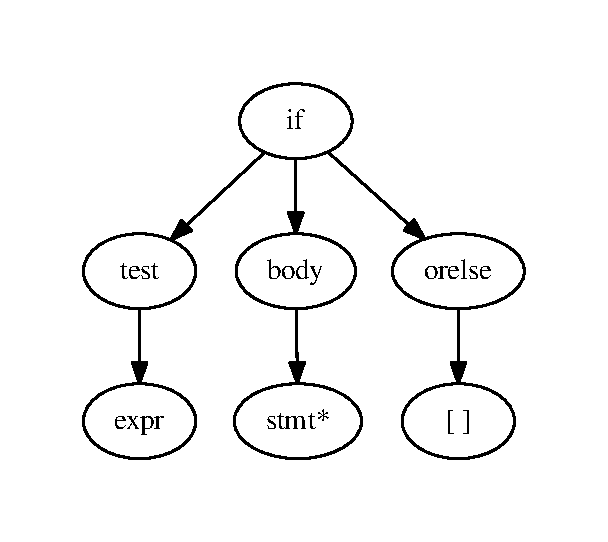
\includegraphics[width=\textwidth]{./figures/dot_files/if_ast.pdf}
    \end{subfigure}
    ~ %add desired spacing between images, e. g. ~, \quad, \qquad, \hfill etc. 
    %(or a blank line to force the subfigure onto a new line)
    \begin{subfigure}[b]{0.45\textwidth}
        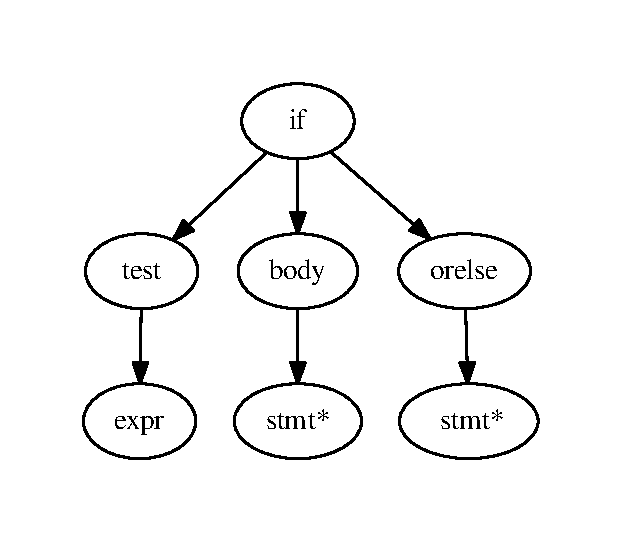
\includegraphics[width=\textwidth]{./figures/dot_files/if_else.pdf}
    \end{subfigure}
    \caption{Abstract graph showing the nodes in the abstract syntax tree for a single \texttt{if} statement on the left and an \texttt{if} and \texttt{else} statement on the right}
    \label{test:ast:if_and_else}
\end{figure}

\begin{figure}
  \centering
  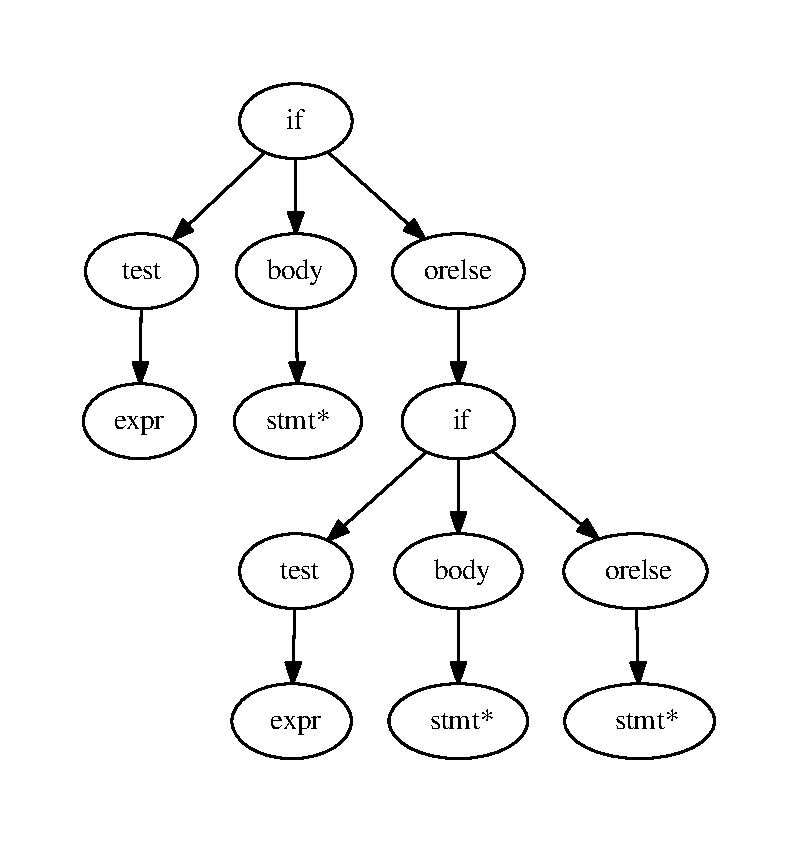
\includegraphics[scale=.7]{./figures/dot_files/if_elif_else.pdf}
  \caption{Abstract graph showing the nodes in the abstract syntax tree for an \texttt{if},\texttt{elif} and \texttt{else} statement}
  \label{test:ast:if_elif_else}
\end{figure}

When the basic cases of the \texttt{if} is implemented we also need to know that \texttt{if} statements inside the body of an \texttt{if} statement works properly.
When that works we need to consider how to handle \texttt{break}, \texttt{yield} and \texttt{return} statements inside the \texttt{if}.

Testing has greatly helped when exploring and developing these cases, because they explicitly run each case every time the test is run.
This assures that a change fixing one case did not break another case.

\paragraph{Complex features}
The development of python is still ongoing which results in periodic changes to both the grammar and the semantics of the language.
Continuously adding features from both the object oriented and the functional paradigm results in more possibilities but also a more complex internal structure.
This is evident when attempting to generate control flow graphs from the abstract syntax.

One example is that you can assign a list to a tuple, and python will \emph{unpack} and assign the items of the list to the corresponding items of the tuple.
This is possible using the \texttt{*}-operator.
An example is show on \cref{tuple:unpacking}, where x is assigned the value 4 and the tuple y is overwritten with the list [5, 6].
\begin{lstlisting}[style=python, caption={Tuple unpacking}, label=tuple:unpacking]
  x = 1
  y = (2,3)
  x,*y = [4,5,6]
\end{lstlisting}

Generating the control flow graph for expressions like these have given a lot of insight into python, but it has also been a challenge to represent them properly in the control flow graph.
Also here testing has provided useful for keeping track of the parts involved.
The example consists of assignments, a tuple, the star operator and a list in order to show off one concept.
All the concepts both need to work individually and together, and tests have helped ensuring this.

\paragraph{Dynamic types}
Python is a dynamic language which can be unforgiving to debug.
A wrong type returned from a function produces an error in a function somewhere else.
That can result in a big stack trace which can be hard to follow.

When developing with tests a catalogue of small tests are naturally developed.
When introducing an error that breaks more than just the construct at hand, test have helped pinpointing the real cause of the error.
This has sometimes lead to insight that either helped us understand why our implementation was wrong, or why what we expected was not the real outcome.

\paragraph{Integration test}
At last some integration tests were added to ensure that \pyt{} produces the right output for each vulnerability example described in \cref{security_vulnerabilities}.
This helped the process of implementing the vulnerability detection, by pointing out when the detected vulnerabilities changed.
